
Albeit having different looks, most interfaces tend to do the same thing; thus, most of the things we have already covered in the previous section are also valid here. Remember, we are going to change our form of the interaction, not the tool we're actually interacting with.

\begin{tcolorbox}[colback=webgreen!5!white,colframe=webgreen!75!black,title=Note]
Before going any further, check whether the ccmake command is available in your terminal. If not, verify your PATH variable is set correctly and check your installation as well.
\end{tcolorbox}

\subsubsubsection{2.3.1\hspace{0.2cm}Learning how to use ccmake (CMake curses GUI)}

ccmake is a terminal-based graphical user interface (GUI) for CMake, which allows users to edit cached CMake variables. Instead of calling it a GUI, the term terminal user interface (TUI) may suit better since there are no traditional shell UI elements such as windows and buttons. These elements are rendered in the terminal using a text-based interface framework named ncurses.

Since ccmake is a part of the default CMake installation, no extra installation is needed besides CMake. Using ccmake is exactly the same as using CMake in a CLI, except it lacks the ability to invoke build and install steps. The main difference is that ccmake will show a terminal-based graphical interface for editing cached CMake variables interactively. This is a handy tool when you are experimenting with the settings. The status bar of ccmake will display a description for each setting and its possible values.

To start using ccmake, use ccmake instead of cmake in the project configure step. In our example, we will exactly replicate the CLI example we did previously in the Configuring a project via the CLI section:

\begin{tcblisting}{commandshell={}}
ccmake -G "Unix Makefiles" -S . -B ./build
\end{tcblisting}

The following shows an example output for the preceding command:

\begin{center}
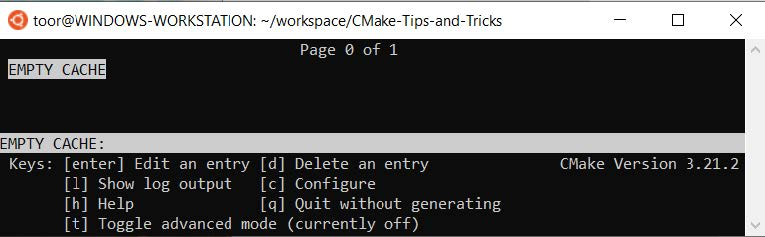
\includegraphics[width=1.\textwidth]{content/1/chapter2/images/23.jpg}\\
Figure 2.23 – ccmake main screen
\end{center}

After running the command, a terminal-based UI will appear. The initial page is the main page where CMake variables can be edited. EMPTY CACHE means no prior configuration has been made and the CMake cache file (CMakeCache.txt) is currently empty. In order to start editing variables, the project must be configured first. To configure, press the C key on the keyboard, as indicated in the Keys: section.

After pressing the C key, the CMake configure step will be executed and the log output screen will be displayed with configuration output:

\begin{center}
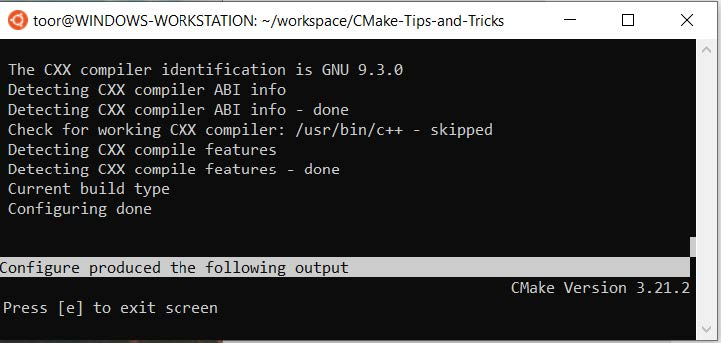
\includegraphics[width=1.\textwidth]{content/1/chapter2/images/24.jpg}\\
Figure 2.24 – ccmake log screen after configuration
\end{center}

To close the log output screen and return to the main screen, press E. Upon return, you will notice that EMPTY CACHE is replaced with variable names in the CMakeCache.txt file. To select a variable, use the up and down arrow keys on your keyboard. The currently selected variable will be highlighted in white, as seen in the next figure:

\begin{center}
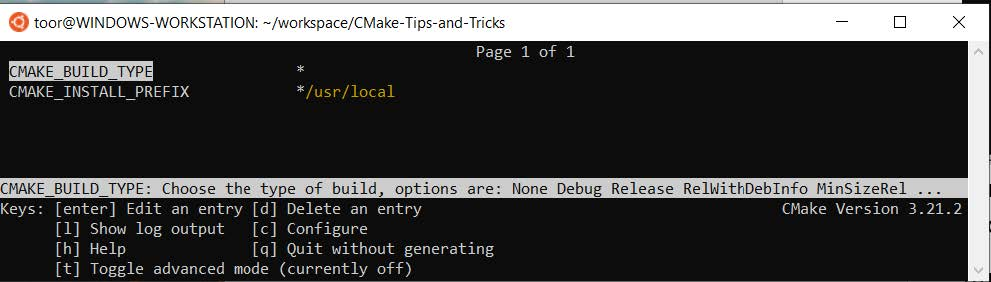
\includegraphics[width=1.\textwidth]{content/1/chapter2/images/25.jpg}\\
Figure 2.25 – ccmake main screen after configuration
\end{center}

In the preceding screenshot, the CMAKE\_BUILD\_TYPE variable is selected. On the righthand side, the current value of the CMake variable is displayed. For CMAKE\_BUILD\_TYPE, it is empty right now. An asterisk next to the value of a variable means that the variable's value has just changed with the prior configuration. You can either edit it by pressing the Enter key or delete it by pressing the D key on the keyboard. The following figure shows what the ccmake main screen looks like after changing the variable:

\begin{center}
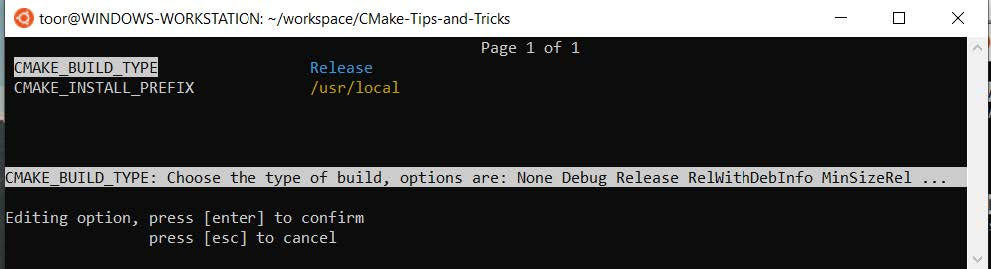
\includegraphics[width=1.\textwidth]{content/1/chapter2/images/26.jpg}\\
Figure 2.26 – ccmake main screen following a variable change
\end{center}

Let's set CMAKE\_BUILD\_TYPE to Release and configure again:

\begin{center}
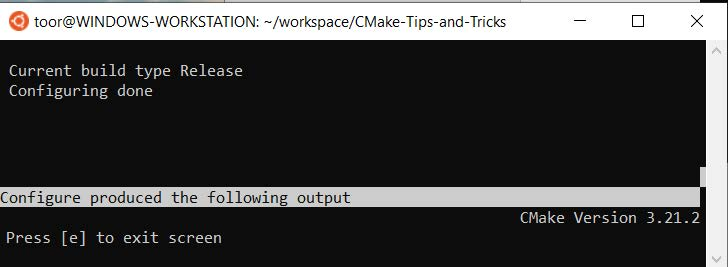
\includegraphics[width=1.\textwidth]{content/1/chapter2/images/27.jpg}\\
Figure 2.27 – ccmake configuration output (Release)
\end{center}

We can observe that the build type is now set to Release. Return to the previous screen and save the changes by pressing the g (generate) button. The changes can be discarded by pressing the q (quit without generating) button.

To edit other variables, such as CMAKE\_CXX\_COMPILER and CMAKE\_CXX\_FLAGS, the advanced mode should be turned on. These variables are, by default, marked as advanced flags by calling the mark\_as\_advanced() CMake function; thus, they are hidden on graphical interfaces by default. On the main screen, press t to toggle to advanced mode.

\begin{center}
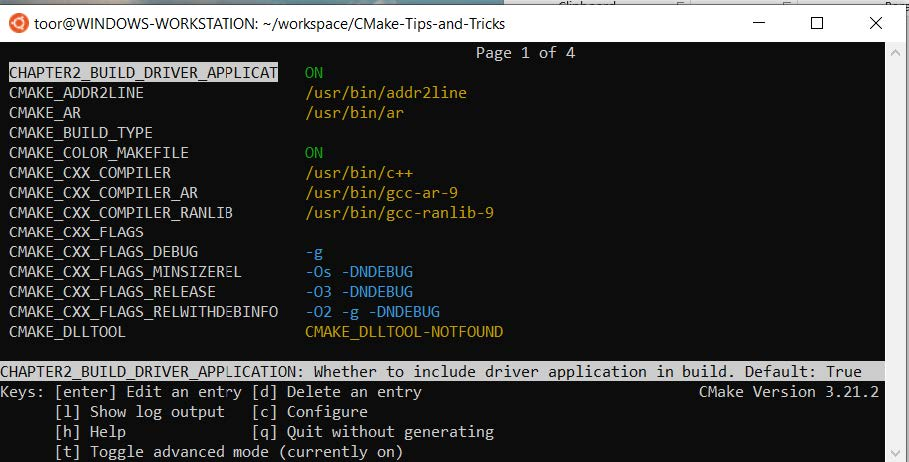
\includegraphics[width=1.\textwidth]{content/1/chapter2/images/28.jpg}\\
Figure 2.28 – ccmake in advanced mode
\end{center}

After activating the advanced mode, a whole new set of options become visible. You can observe and alter their values, just like normal variables. You may have noticed that a previously hidden variable named CHAPTER2\_BUILD\_DRIVER\_APPLICATION is now present. This is a user-defined CMake variable. This variable is defined as follows:

\begin{lstlisting}[style=styleCMake]
# Option to exclude driver application from build.
set(CHAPTER2_BUILD_DRIVER_APPLICATION TRUE CACHE BOOL "Whether
to include driver application in build. Default: True")
# Hide this option from GUI's by default.
mark_as_advanced(CHAPTER2_BUILD_DRIVER_APPLICATION)
\end{lstlisting}

The CHAPTER2\_BUILD\_DRIVER\_APPLICATION variable is defined as a cache variable with a Boolean type, having a default value of true. It is marked as advanced, which is why it was not present in the non-advanced mode.

\subsubsubsection{2.3.2\hspace{0.2cm}Using CMake via cmake-gui}

If you are the type of person who finds CLIs counter-intuitive, or you prefer GUI over CLI, CMake has a cross-platform GUI, too. In contrast to ccmake, cmake-gui has more to offer, such as Environment Editor and Regular Expression Explorer.

The CMake GUI is a part of the default CMake installation; no extra installation is needed besides CMake. Its main purpose is to allow a user to configure a CMake project. To launch cmake-gui, issue the cmake-gui command in your terminal. For Windows, it can be also located from the start menu. If none of these methods work, go into your CMake installation path and it should be present in the bin\ directory

\begin{tcolorbox}[colback=webgreen!5!white,colframe=webgreen!75!black,title=Note]
If you are launching cmake-gui in a Windows environment and you intend to use the toolchain provided by Visual Studio, launch cmake-gui from the appropriate Native Tools Command Prompt of your IDE. If you have multiple versions of IDEs, ensure that you are using the correct Native Tools Command Prompt. Otherwise, CMake may fail to discover the required tools, such as a compiler, or may find incorrect ones. Refer to \url{https://docs.microsoft.com/en-us/visualstudio/ide/reference/command-prompt-powershell?view=vs-2019} for further information.
\end{tcolorbox}

Here is the main window of the CMake GUI:

\begin{center}
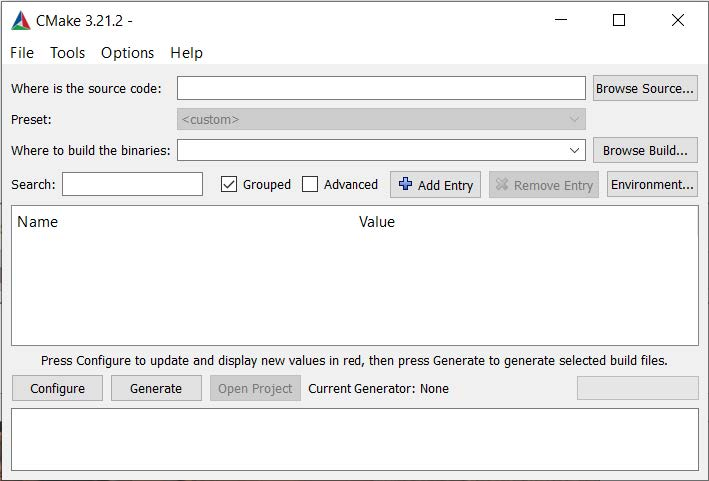
\includegraphics[width=1.\textwidth]{content/1/chapter2/images/29.jpg}\\
Figure 2.29 – CMake GUI main window
\end{center}

The main screen of the CMake GUI essentially contains the following:

\begin{itemize}
\item 
Source code path field

\item 
Output path field

\item 
Configure and generate buttons

\item 
Cache variable list
\end{itemize}

These are the four essential things we are going to interact with. To start configuring a project, select the project's root directory by clicking the Browse Source… button. Consequently, select an output directory for the project by clicking the Browse Build… button. This path will be the path for the generated output files by the selected generator.

After setting source and output paths, click Configure to start configuring the selected project. The CMake GUI will let you choose details such as the generator to be used, platform selection (if supported by the generator), toolset, and compiler, as shown in the following figure:

\begin{center}
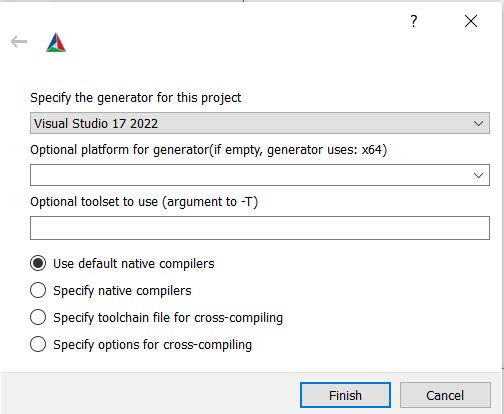
\includegraphics[width=1.\textwidth]{content/1/chapter2/images/30.jpg}\\
Figure 2.30 – CMake GUI generator selection screen
\end{center}

After filling in these details according to your environment, click Finish to continue. The CMake GUI will start configuring your project with the given details and report the output in the log section. Upon successful configuration, you should also see the cache variables in the cache variable list section as well:

\begin{center}
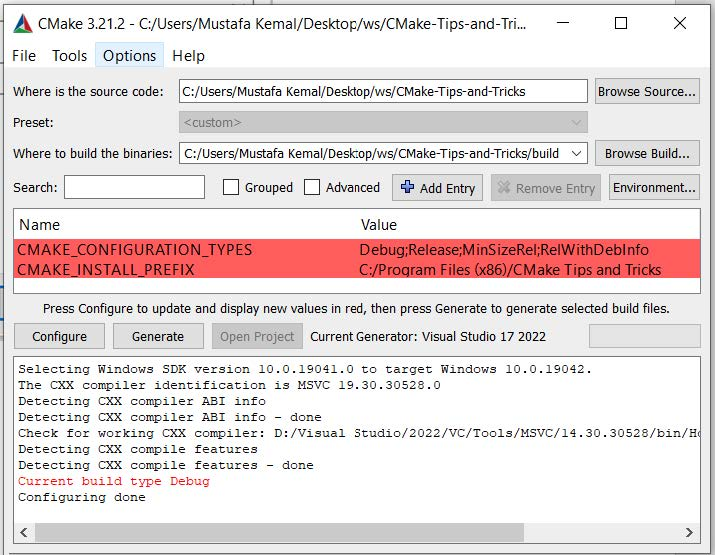
\includegraphics[width=1.\textwidth]{content/1/chapter2/images/31.jpg}\\
Figure 2.31 – CMake GUI after configuration
\end{center}

If everything seems to be in order, press the Generate button to generate the build files that are needed by the build system of your choice. For Visual Studio generators, the generated files are .sln and .cxxproj along with other stuff. After generating the project, the Open Project button will become enabled. It will cause the generated project to be opened with the appropriate editor or IDE. If the build system is not associated with any IDE (for example, makefiles), then generated files will be displayed instead. After that, you can use your IDE to build the project.

\begin{tcolorbox}[colback=webgreen!5!white,colframe=webgreen!75!black,title=Important Note]
Be aware that the generated project is just the generator's artifact, and changes to the generated project files (.sln, .cxxproj) will not be saved and will be lost on the next generation. Don't forget to regenerate project files when you  make a change to the CMakeLists.txt files or edit a CMakeCache. txt file (either directly or indirectly). For the version-control aspect, you should treat generated project files as build artifacts and should not add them to version control. You can always obtain them from scratch by generating the project with an appropriate generator via CMake.
\end{tcolorbox}

Sometimes, a project may need tweaking some cache variables or you may decide to use a different build type, for example. To change any cache variables, click on the value of the desired cache variable; it should become editable. Depending on the variable type, a checkbox may be displayed instead of a string. If the desired variable is not visible on the list, it may be an advanced variable, which can only be visible when the Advanced checkbox on the window is checked. You can also use the search box to locate the variable with more ease. Here, you can see cmake-gui in Advanced Mode:

\begin{center}
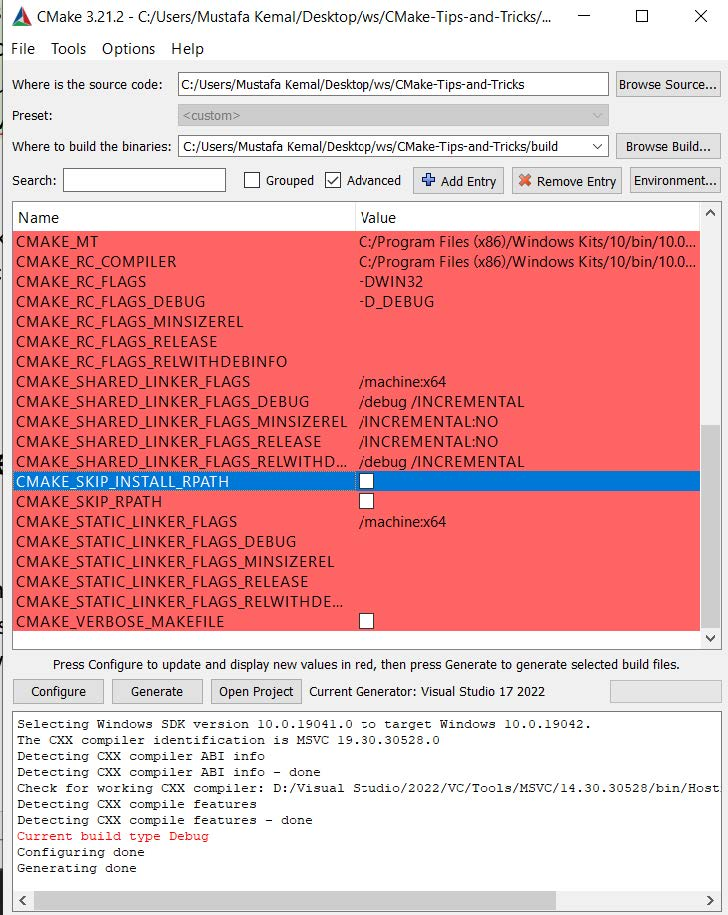
\includegraphics[width=1.\textwidth]{content/1/chapter2/images/32.jpg}\\
Figure 2.32 – cmake-gui in advanced mode
\end{center}

After tweaking any cache values, click Configure and then Generate to apply the changes.

\begin{tcolorbox}[colback=webgreen!5!white,colframe=webgreen!75!black,title=Tip]
Another useful feature is the grouping feature, which allows the grouping of cache variables into their common prefix, if there is one. Group names are determined by the first part of the variable name, up to the first underscore.
\end{tcolorbox}

We have covered the most essential features of cmake-gui. Before moving to other miscellaneous stuff, if you ever need to reload cache values or delete the cache and start from scratch, you can find the Reload Cache and Delete Cache menu items in the File menu.

\subsubsubsection{2.3.3\hspace{0.2cm}Tweaking environment variables}

The CMake GUI comes with a handy environment variable editor that allows CRUD operations on environment variables. To access it, simply click the Environment… button on the main screen. After clicking, the Environment Editor window will pop up, as can be seen in the following figure:

\begin{center}
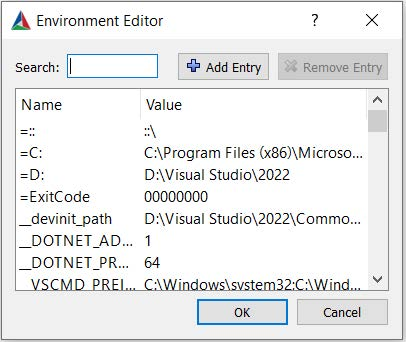
\includegraphics[width=0.8\textwidth]{content/1/chapter2/images/33.jpg}\\
Figure 2.33 – CMake GUI environment variable editor
\end{center}

The Environment Editor window contains a list of the environment variables present in the current environment. To edit an environment variable, double-click on the value field of the desired environment variable in the table. The window also allows information to be added and deleted with the Add Entry and Remove Entry buttons.

\subsubsubsection{2.3.4\hspace{0.2cm}Evaluating regular expressions with CMake}

Have you ever wondered how a regular expression would get evaluated by CMake and what results it would give exactly? If so, you may have previously debugged it manually by printing out the regex match result variables with message(). What if I say there is a better way to do it? Let me introduce you to the Regular Expression Explorer tool of the CMake GUI.

\begin{center}
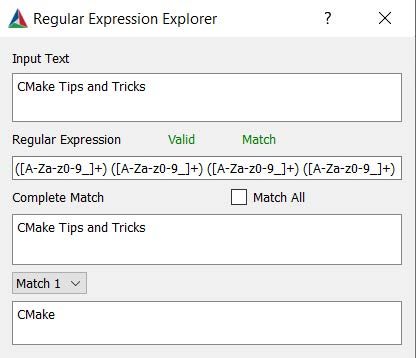
\includegraphics[width=0.8\textwidth]{content/1/chapter2/images/34.jpg}\\
Figure 2.34 – CMake GUI Regular Expression Explorer
\end{center}

This hidden gem allows you to debug regular expressions using CMake's regex engine. It is located in the Tools menu with the name Regular Expressions Explorer…. Using it is pretty simple and straightforward:

\begin{enumerate}
\item 
Enter the expression in the Regular Expression field.

The tool will check whether the expression is valid. If so, the Valid text on the screen will be green. It will turn red if CMake's regex engine did not like the expression you've given.

\item 
Enter the test string in the Input Text field. The regular expression will be matched against this text.

\item 
If there is any match, the Match word on the window will turn from red to green. The matching string will be printed in the Complete Match field.

\item 
On matching, capture groups will be assigned to Match 1, Match 2, to Match N, respectively, if any.
\end{enumerate}

In this section, we've learned how to use CMake's native graphical interfaces. We will continue learning about using CMake by taking a look at a selection of CMake's IDE and editor integrations next.
